\include{template}
%\cfoot{} %% if no page number is needed

\begin{document}

\begin{header}
FICHE TECHNIQUE

Le banc Kofler
\end{header}

\begin{figure}[h]
\begin{center}
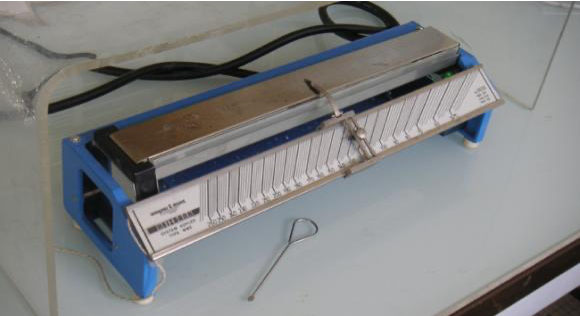
\includegraphics[height=190pt]{images/banc_kofler.png}
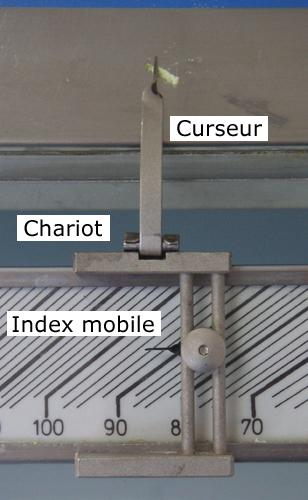
\includegraphics[height=190pt]{images/banc_kofler_chariot.jpg}
\end{center}
\end{figure}

Le banc Kofler est une plaque chauffante sur laquelle s'établit une élévation régulière de température.
Il permet de mesurer précisément la température de fusion d'un solide.

La vidéo \href{https://tinyurl.com/yxsvz6e7}{https://tinyurl.com/yxsvz6e7} démontre l'utilisation du banc Kofler (regarder à partir de 2'17'').

\section*{Précautions}

\begin{itemize}
\item[•] \textbf{La manipulation sera notée : appeler le professeur !}
\item[•] Le banc Kofler doit être branché depuis au moins une demi-heure avant de faire la mesure.
\item[•] Ne pas porter de gants lors de l'utilisation du banc Kofler.
Ils pourraient fondre et causer de graves brulures.
\item[•] Ne pas \og bruler \fg{} les substances en allant vers les températures trop élevées.
\item[•] N'utiliser que de très \small très \footnotesize très \scriptsize très \tiny très \normalsize petites quantités de solide pour chaque mesure.
\item[•] Le banc Kofler doit être étalonné pour donner une valeur précise.
\end{itemize}

\section*{Mesure}

\begin{enumerate}
\item Déposer une pointe de spatule de solide dans une zone de température inférieure à sa température de fusion.
\item Déplacer lentement le solide vers la zone chaude du banc avec la pointe de la spatule.
\item Repérer la température de fusion à l'apparition de la première goutte de liquide.
\item Déplacer horizontalement le chariot jusqu'à ce que le curseur soit à la frontière entre solide et liquide.
\item Lire la valeur indiquée par l'index mobile.
\item Nettoyer le banc Kofler comme décrit plus bas.
\end{enumerate}

\section*{Nettoyage}

La manipulation n'est pas complète sans le nettoyage du banc Kofler.
\begin{enumerate}
\item À l'aide d'un petit morceau de coton, éliminer le solide en le poussant vers la zone froide du banc Kofler.
\item Avec un morceau de coton imbibé d'éthanol, répéter l'opération pour éliminer toute résidu.
Un seul passage est suffisant !
\end{enumerate}

\end{document}